
%(BEGIN_QUESTION)
% Copyright 2015, Tony R. Kuphaldt, released under the Creative Commons Attribution License (v 1.0)
% This means you may do almost anything with this work of mine, so long as you give me proper credit

\noindent
{\bf Laboratorieøvelse -- introduksjon}

\vskip 5pt

Oppgaven deres er å legge til kaskade-, forholds- eller feedforward-regulering i det fungerende prosessreguleringssystemet. Dette krever at dere legger til en ekstra prosesstransmitter, samt ekstra programmering i regulatoren.

Tabellen under viser mål dere og teamet må fullføre innen avsatt tid for denne laboratorieøvelsen. Merk at noen mål er individuelle, mens andre gjelder teamet som helhet:

\underbar{Tabell for måloppnåelse:}

% No blank lines allowed between lines of an \halign structure!
% I use comments (%) instead, so that TeX doesn't choke.

$$\vbox{\offinterlineskip
\halign{\strut
\vrule \quad\hfil # \ \hfil & 
\vrule \quad\hfil # \ \hfil & 
\vrule \quad\hfil # \ \hfil & 
\vrule \quad\hfil # \ \hfil & 
\vrule \quad\hfil # \ \hfil & 
\vrule \quad\hfil # \ \hfil & 
\vrule \quad\hfil # \ \hfil \vrule \cr
\noalign{\hrule}
%
% First row
{\bf Ytelsesmål} & {\bf Vurdering} & {\bf 1} & {\bf 2} & {\bf 3} & {\bf 4} & {\bf Team} \cr
%
\noalign{\hrule}
%
% Another row
Godkjenning av reguleringsstrategi & mestring & -- & -- & -- & -- & \cr
%
\noalign{\hrule}
%
% Another row
Teammøte og prototypeskisse & mestring & -- & -- & -- & -- & \cr
%
\noalign{\hrule}
%
% Another row
Kretsdesign-utfordring & mestring & & & & & -- -- -- -- \cr
%
\noalign{\hrule}
%
% Another row
Endelig sløyfediagram og systeminspeksjon & mestring & & & & & -- -- -- -- \cr
%
\noalign{\hrule}
%
% Another row
P\&ID som viser reguleringsstrategi & mestring & & & & & -- -- -- -- \cr
%
\noalign{\hrule}
%
% Another row
Demonstrasjon av fungerende system & mestring & -- & -- & -- & -- & \cr
%
\noalign{\hrule}
%
% Another row
Labspørsmål: Instrumentkoblinger & proporsjonal &  &  &  &  & -- -- -- -- \cr
%
\noalign{\hrule}
%
% Another row
Labspørsmål: Idriftsettelse & proporsjonal &  &  &  &  & -- -- -- -- \cr
%
\noalign{\hrule}
%
% Another row
Labspørsmål: Hoderegning & proporsjonal &  &  &  &  & -- -- -- -- \cr
%
\noalign{\hrule}
%
% Another row
Labspørsmål: Diagnostikk & proporsjonal &  &  &  &  & -- -- -- -- \cr
%
\noalign{\hrule}
} % End of \halign 
}$$ % End of \vbox

Den eneste ``proporsjonale'' vurderingen i denne aktiviteten er labspørsmålene, som besvares individuelt av hver student. En liste over mulige labspørsmål finnes på slutten av denne oppgaven. Spørsmålene er ment både som læringsstøtte og vurdering, og kan derfor bli stilt av instruktøren fortløpende gjennom labperioden, ikke nødvendigvis samlet på én dag.

\vskip 10pt

{\bf Det er avgjørende at teamet planlegger hva som skal oppnås hver dag. Et kort (10 minutter) teammøte ved starten av hver labøkt er en god arbeidsform: gå gjennom hva som er gjort, hva som gjenstår, og hvilke vurderinger dere må være forberedt på. Det er mye arbeid i å bygge, dokumentere og feilsøke fungerende instrumentsystemer!}

Når dere arbeider med systemet, vil det uunngåelig oppstå problemer. Forsøk alltid å løse problemene som team før dere ber instruktøren om hjelp. Hvis dere fortsatt trenger hjelp, skriv teamfargen deres på lab-tavlen sammen med en kort beskrivelse av hva dere trenger hjelp til. Instruktøren følger opp teamene i den rekkefølgen de står på tavlen.





\vfil \eject

\noindent
{\bf Laboratorieøvelse -- endring av reguleringsstrategi}

\vskip 5pt

Første steg er å bestemme hvilken flerinngangsstrategi dere skal implementere. Både kaskade og feedforward brukes for å redusere påvirkningen fra forstyrrelser i prosessen, mens forholdsregulering brukes for å låse én prosessvariabel til en annen. Forholdsregulering er ofte enklest å implementere, men passer ikke alltid for studentbygde prosesser. Kaskaderegulering brukes ofte på strømning gjennom reguleringsventilen, noe som kan være krevende å måle med tilgjengelig instrumentering. Feedforward er ofte lett å finne anvendelser for, men kan være krevende å tune riktig. En praktisk anbefaling er å velge feedforward: da lærer dere ofte mest.

For eksempel, her er et enkelt trykkreguleringssystem for luft med sløyferegulator:

$$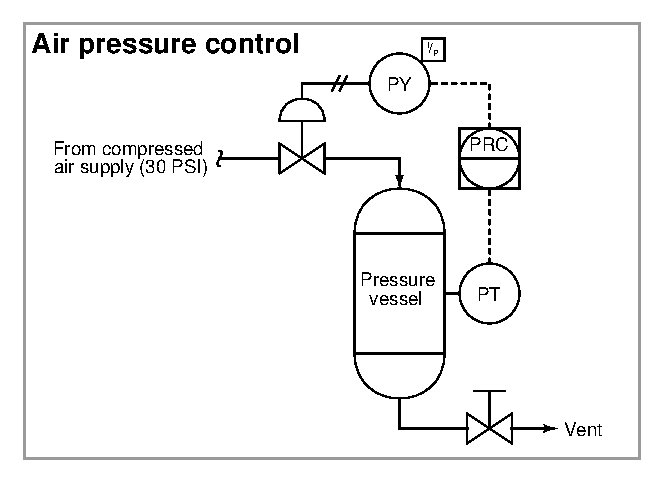
\includegraphics[width=15.5cm]{i00921x03.eps}$$

Deretter ser vi systemet modifisert for kaskaderegulering (ekstra elementer i rødt):

$$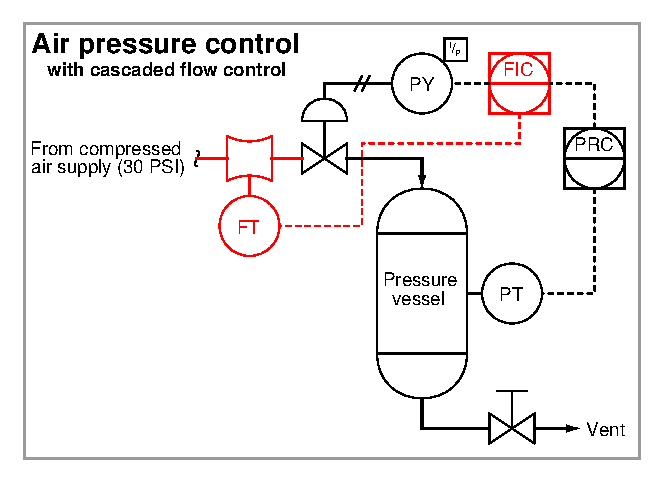
\includegraphics[width=15.5cm]{i00921x01.eps}$$

\filbreak

I neste eksempel ser vi samme grunnsystem modifisert for feedforward-regulering (ekstra elementer i rødt):

$$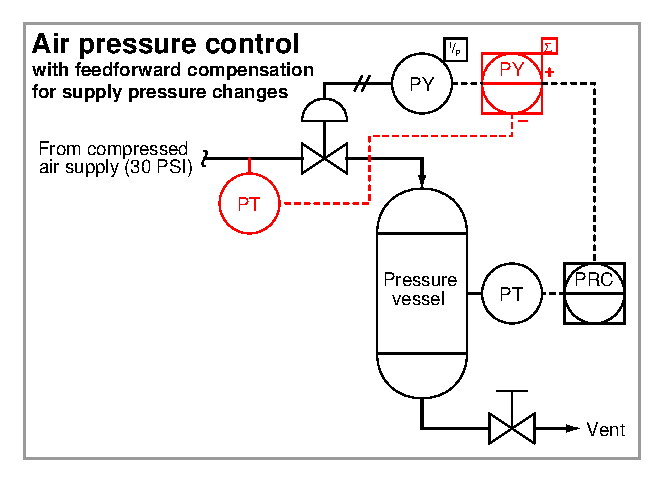
\includegraphics[width=15.5cm]{i00921x02.eps}$$


Etter valg av strategi bør neste steg være å velge riktig måleinstrument for den ekstra variabelen, lage en prototypetegning som viser hvordan instrumentet integreres i eksisterende system, og deretter installere instrumentet i prosessen. Som vanlig er prototypeskissen så viktig at instruktøren krever den før bygging av det fungerende systemet starter. {\it Team som endrer reguleringsstrategi uten verifisert plan vil bli stoppet og får ikke fortsette før en prototypeløsning er laget og godkjent!} Hvert teammedlem bør ha enkel tilgang til planen under byggingen.

Installasjonen skal følge samme standard som i den opprinnelige konstruksjonen: kabling i føring der det er mulig, ryddig tubing, og tydelig merking av instrumenter og kabler med ISA-standard tag-navn. Etter installasjon bør ny transmitter testes for å verifisere forventet måling. Regulatorens visning av den nye variabelen skal være korrekt skalert i ingeniørenheter, ikke bare prosent.

Hvis transmitteren måler riktig, er neste steg å utforme regulatorprogrammet som bruker de nye prosessdataene til å stabilisere den opprinnelige prosessvariabelen. Detaljene varierer mye. Læreboken {\it Lessons In Industrial Instrumentation} beskriver kaskade, forhold og feedforward i detalj. Instruktøren kan også hjelpe med en praktisk strategi.

\vskip 10pt

{\bf Vanlige feil:}

\begin{itemize}
\item{} Å ikke konsultere produsentdokumentasjon for feltinstrumenter (f.eks. kobling og kalibrering).
\item{} Å montere feltinstrumenter på uhensiktsmessige steder, slik at tilkoblinger og deksler blir vanskelige å komme til.
\item{} Feil montering av rør-/tubingkoblinger (f.eks. blanding av fittings som ikke passer sammen).
\item{} Å unnlate å trekkteste hver leder i terminalen for å sikre mekanisk god forbindelse.
\item{} At studenter jobber isolert uten å dele med teamet hva som er gjort og hvorfor.
\end{itemize}





\vfil \eject

\noindent
{\bf Laboratorieøvelse -- teammøte, prototypeskisse og instrumentvalg}

\vskip 5pt

Et viktig første steg er å {\bf møte instruktøren} som team for å diskutere sikkerhet, teamytelse og roller. Hvis dere vil prioritere erfaring med bestemt utstyr, teknikker eller oppgaver, er dette riktig tidspunkt for å avklare det i teamet.

\vskip 10pt

Et helt sentralt steg er å samarbeide om å {\bf skissere et prototype-diagram} av det dere skal bygge. Dette er ofte et enkelt koblingsskjema og/eller sløyfediagram med alle elektriske forbindelser, samt tubing/rør for medier. Skissen trenger ikke være uttømmende, men må ha nok detaljer til at instruktøren kan vurdere sikker og riktig funksjon.

Hvis dere for eksempel kobler feltenheter til en PLC, må skissen vise hvordan enhetene kobles til I/O-terminaler, hvor strømforsyning kommer fra osv. Skissen trenger ikke vise alle mellomliggende koblinger, som terminalblokker i koblingsbokser.

Bruk gode problemløsningsmetoder når skissen lages: slå opp i manualer, marker strømretninger, polariteter og identifiser kilder/laster. Se på dette som trening i analyseferdigheter. Husk at dere på sikt skal gjøre dette selvstendig.

Prototypeskissen er så viktig at instruktøren krever den før bygging starter. {\it Team som bygger uten verifisert plan vil bli stoppet til planen er laget og godkjent!} Ikke avvik fra planen uten instruktørgodkjenning.

\vskip 10pt

{\bf Planlegging av et fungerende system bør ta under én time ved effektivt teamarbeid, og kan spare mange timer frustrasjon (og mulig komponentskade).}





\vfil \eject

\noindent
{\bf Laboratorieøvelse -- utfordring i kretsdesign}

\vskip 5pt

Koble et ``ice-cube''-relé til en lavspenning DC-kilde og samtidig til 120 V AC, slik at en håndbetjent bryter på lavspenning DC styrer innkobling av en 120 VAC-last. Alle elektriske forbindelser skal utføres via rekkeklemme (ingen tvinnede ledere, klemmer, wire nuts eller krokodilleklemmer), og 120 VAC-delen skal sikres mot overstrøm.

Øvelsen tester evnen til å tolke pinout for elektromekanisk relé, koble bryter til reléspole, koble last til relékontakter, velge NO/NC-kontakter riktig, og bruke rekkeklemme til ryddig oppbygging.

$$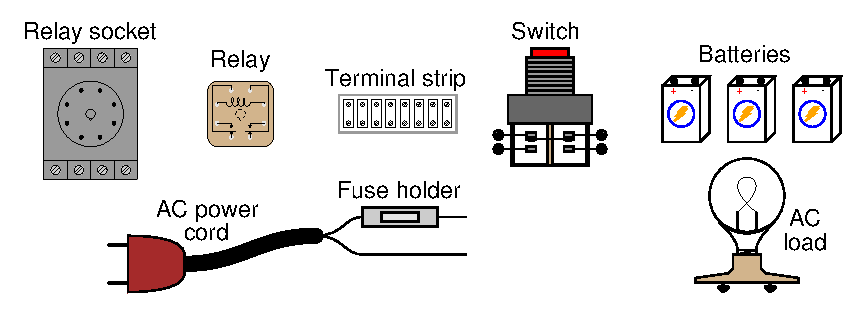
\includegraphics[width=15.5cm]{i00921x04.eps}$$

\vskip 10pt

Følgende komponenter/materialer er tilgjengelige: ulike ``ice cube'' {\bf reléer} med DC-spoler og matchende {\bf sokler}; ulike trykknapp-{\bf brytere}; {\bf rekkeklemmer}; {\bf koblingsledning}; {\bf batteriklemmer}; 120 VAC {\bf nettkabel} med {\bf sikringsholder}; 120 VAC {\bf lampe eller annen passende last}.

\vskip 10pt

Dere må selv ha skrutrekkere og multimeter for montering og test ved arbeidsplassen. Instruktøren leverer batteri(er) når kretsen er klar for funksjonstest. Inntil da skal kretsen være spenningsløs.

\vskip 20pt

\noindent
{\bf Last-/bryterstatus} (instruktør velger): \hskip 20pt \underbar{\hskip 20pt} På når trykket \hskip 10pt {\it eller} \hskip 10pt \underbar{\hskip 20pt} Av når trykket

\vfil

Studer referansen: ``Control Relays'' i {\it Lessons In Industrial Instrumentation}.





\vfil \eject

\noindent
{\bf Laboratorieøvelse -- dokumentasjon av systemet}

\vskip 5pt

Hver student skal lage eget {\it sløyfediagram} for teamets system etter ISA-konvensjoner. Diagrammet skal være en utvidelse av opprinnelig PID-sløyfe og vise ny transmitter koblet til sløyferegulatoren.

Som vanlig skal sløyfediagrammet være {\it komplett} og {\it detaljert}: alle ledere, kabler, terminaler, områder osv. Målet er at en uten forhåndskunnskap skal kunne følge diagrammet og koble riktig.

Alle instrumenter og signalkabler skal merkes med ISA-standard tag-nummer. En enkel metode er maskeringstape med permanent tusj på hver kabel og hvert instrument. En praktisk anbefaling er å merke hver 2-lederkabel med taggen til feltinstrumentet den går til.

Når teamet er ferdig med individuelle sløyfediagrammer, tilkall instruktør for inspeksjon. Da går studentene gjennom sløyfen etter tur, mens resten av teamet kontrollerer diagrammer for feil og mangler. Installasjonskvalitet vurderes også (ledere, terminering, kabelruting, merking osv.). Teamet må rette avvik for å få godkjent systemet.

Etter godkjent inspeksjon skal hvert teammedlem legge sløyfediagrammet i diagramholderen i laben bak hovedpanelet. Ved feilsøking av andre team sitt system henter dere diagrammet der.

\vskip 10pt

I tillegg til modifisert sløyfediagram må dere levere et printet diagram av regulatorens nye algoritme, vanligvis som funksjonsblokkdiagram. Brukes DCS, kan dette være skjermbilde fra funksjonsblokk-editor.

Funksjonsblokkdiagrammet er kritisk for diagnostikk. Sløyfediagrammet dokumenterer koblinger, men viser ikke reguleringsstrategien i seg selv.

\vskip 10pt

{\bf Vanlige feil:}

\begin{itemize}
\item{} Glemme å merke alle signalledere.
\item{} Glemme å merke alle feltinstrumenter med tag-navn (f.eks. PT-83).
\item{} Glemme å notere alle lederfarger.
\item{} Glemme å skrive navn på sløyfediagrammet.
\item{} Basere eget diagram på en lagkamerats i stedet for å inspisere systemet selv.
\item{} Plassere instrumenter feil i sløyfearket (felt til venstre, kontrollrom til høyre).
\end{itemize}

\vskip 10pt

{\bf Korrekt utarbeidelse og inspeksjon av sløyfediagrammer bør ved effektivt teamarbeid kunne gjøres på maksimalt én full labøkt (3 timer).}





\vfil \eject

\noindent
{\bf Laboratorieøvelse -- tuning av reguleringsstrategi}

\vskip 5pt

Forholdsregulering er vanligvis enklest å tune: settpunktet byttes fra ``local'' til ``remote'', eventuelt med en ratio-funksjonsblokk for skalering av den frie variabelen til den bundne. Hvis opprinnelig sløyfe var godt tunet, trenger PID-innstillingene ofte ikke endres.

\vskip 10pt

Kaskaderegulering innebærer vanligvis en ekstra PID-funksjon (ofte i samme regulator). ``Slave'' må tunes før ``master'' tunes. Merk at opprinnelig PID (nå master) kan trenge retuning etter overgang til kaskade, fordi prosessdynamikken sett av master ofte endres.

\vskip 10pt

Feedforward er ofte mest krevende å justere, spesielt med dynamisk kompensasjon. Prinsippet er å reagere proaktivt på lastendringer, slik at feedback-regulatoren ikke trenger å korrigere i etterkant. For å evaluere feedforward settes feedback-regulator i manuell, deretter introduseres lastendring. Dersom feedforward er riktig skalert, får lastendringen liten effekt på PV selv med PID i manuell.

En feedforward-løkke som er for aggressiv overkompenserer. En som er for svak lar lastendringer gi tydelig PV-utslag. Aggressivitet justeres med {\it gain} i en gain/bias-funksjonsblokk mellom feedforward-sensor og summerblokk.

Hvis feedforward til slutt kompenserer, men med tydelig forbigående PV-avvik, trengs ofte {\it dynamisk kompensasjon} i form av {\it lead/lag} eller {\it dead time}. Juster disse først etter at gain/bias er riktig tunet i stasjonær tilstand.





\vfil \eject

\noindent
{\bf Labspørsmål}

\vskip 5pt

\begin{itemize}
\item{} {\bf Instrumentkoblinger}
\item{} Bestem riktige lederkoblinger mellom instrumenter for å etablere fungerende 4-20 mA sløyfe ut fra instrumentdiagram med merkede terminaler
\item{} Identifiser korrekt alle elektriske kilder og laster, samt polariteter og strømretninger i en 4-20 mA sløyfe
\end{itemize}

\filbreak

\begin{itemize}
\item{} {\bf Idriftsettelse og dokumentasjon}
\item{} Gi et praktisk eksempel på {\it forholdsregulering} og forklar virkemåte
\item{} Gi et praktisk eksempel på {\it kaskaderegulering} og forklar virkemåte
\item{} Gi et praktisk eksempel på {\it feedforward-regulering} og forklar virkemåte
\item{} Gi et praktisk eksempel på {\it selector}-regulering og forklar virkemåte
\item{} Gi et praktisk eksempel på {\it override}-regulering og forklar virkemåte
\item{} Angi riktig rekkefølge for tuning av begge PID-regulatorer i kaskade og forklar hvorfor
\item{} Beskriv hvordan man ser at et feedforward-system er riktig tunet i drift
\item{} Forklar trinnvis hvordan en regulator i automatisk modus kan sikres for kalibrering av primærtransmitter uten prosesstans
\item{} Forklar trinnvis hvordan en regulator i automatisk modus kan sikres for kalibrering av sekundærtransmitter uten prosesstans
\item{} Forklar trinnvis hvordan en regulator i automatisk modus kan sikres for slagtest/kalibrering av reguleringsventil uten prosesstans
\end{itemize}

\filbreak

\begin{itemize}
\item{} {\bf Hoderegning} (ingen kalkulator!)
\item{} Beregn pneumatisk trykk i 3-15 PSI-område tilsvarende $x$ prosent
\item{} Beregn elektrisk strøm i 4-20 mA-område tilsvarende $x$ prosent
\item{} Beregn elektrisk spenning i 1-5 V-område tilsvarende $x$ prosent
\item{} Beregn prosentverdi av pneumatisk trykksignal $x$ PSI i 3-15 PSI-område
\item{} Beregn prosentverdi av elektrisk strømsignal $x$ mA i 4-20 mA-område
\item{} Beregn prosentverdi av elektrisk spenningssignal $x$ V i 1-5 V-område
\end{itemize}

\filbreak

\begin{itemize}
\item{} {\bf Diagnostikk}
\item{} Forklar hvordan man skiller ``åpen'' kabel-feil fra ``kortsluttet'' kabel-feil med kun voltmeter (uten strøm-/motstandsmåling)
\item{} Forklar bruk av regulatorens ``manual''-modus som diagnostisk test for kontrollsystemfeil
\item{} Vurder om en gitt diagnostisk test gir nyttig informasjon for et gitt symptomsett
\item{} Oppgi minst to plausible feil gitt testresultater og symptomer
\item{} Foreslå en diagnostisk test og forklar betydningen av to ulike mulige testresultater
\end{itemize}

\underbar{file i00921}
%(END_QUESTION)





%(BEGIN_ANSWER)


%(END_ANSWER)





%(BEGIN_NOTES)

\noindent
{\bf Sløyfediagrammer / inspeksjoner:}

Jeg anbefaler sterkt å krysse av studentenes sløyfediagrammer mens dere inspiserer sløyfen (sikker kabling, tubing, føringsvei osv.). La alle teammedlemmer ta deg med på en ``runde'' i den ferdige sløyfen, der hvert medlem forklarer en del av sløyfen ved hjelp av eget diagram. Mens en student forklarer, kan du kontrollere de andres diagrammer for nøyaktighet.

\vskip 10pt

\goodbreak

\noindent
{\bf Ideer til feilsøkingsfeil:}

\begin{itemize}
\goodbreak
\item{} Avisoler leder i terminal, men stram på isolasjonen (åpen-leder-feil)
\item{} Kutt signalkabel et sted i rørføringen (åpen-leder-feil)
\item{} Stikk tegnestift gjennom kabel i rørføring (kortslutningsfeil)
\item{} Bytt om lederne i instrumentkabel (konstruksjonsfeil)
\item{} Sett for høy demping i transmitter (treg respons)
\item{} Sett for høy demping i indikator/regulator (treg respons)
\item{} Feilkalibrer transmitter og/eller indikator/regulator (unøyaktighet)
\item{} Tett tubing med skumpropp i fittings (treg respons)
\item{} Reverser virkemåte på regulator/positioner/transmitter (feil respons)
\item{} Feilkonfigurer lineær/kvadratrot-karakterisering (ikke-linearitet)
\item{} Koble 2.2 k motstand parallelt med 4-20 mA-transmitter (delvis kortslutning)
\item{} Bytt 250 ohm motstand med feil verdi som ser lik ut (unøyaktighet)
\item{} Koble fra kabel internt i transmitter eller regulator (instrumentfeil)
\item{} Gi studentene feil sløyfediagram (dokumentasjonsfeil)
\item{} La studentene starte på feil regulator (operatørfeil)
\item{} Steng ventil og la sikkerhetsmerking henge på (operatør-/teknikerfeil)
\end{itemize}










\vfil \eject

\noindent
{\bf Labspørsmål}

\vskip 20pt

\begin{itemize}
\item{} Skisser lederkoblinger som gjør dette til et fungerende kontrollsystem. Du skal kun skissere {\it ledninger}, ingen ekstra komponenter er nødvendig:

$$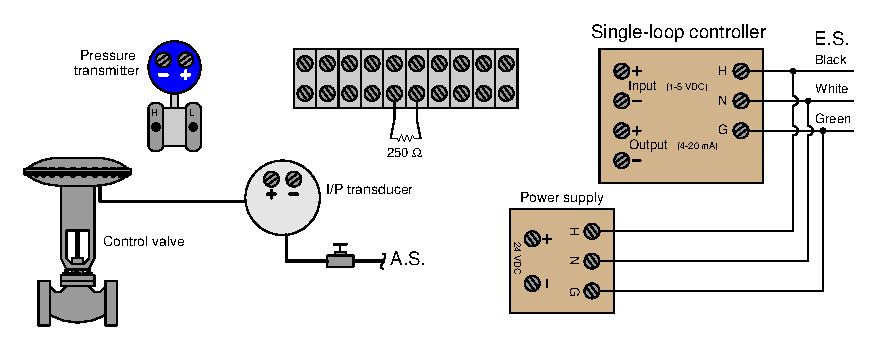
\includegraphics[width=15.5cm]{i00921x06.eps}$$ 

\vskip 20pt

\item{} Beskriv en praktisk anvendelse av {\it selector}-regulering og forklar hvordan den virker.

\vskip 20pt

\item{} Beregn elektrisk spenning i området 1-5 V ved 65 prosent.

\vskip 20pt

\item{} Det er et problem i kontrollsystemet under for matesumpen til en anaerob råtnetank som produserer metangass fra husdyrgjødsel og matavfall. Operatøren rapporterer høy væskenivåvisning på LI-5 (8 fot 11 tommer), selv om pumpen (P-1) går som den skal. En tekniker foreslår manuell nivåmåling med ``dipstick'' gjennom lufting for å verifisere LI-5. Forklar hva testen forteller om feilens art og plassering dersom (1) målingen bekrefter høyt nivå, og (2) dersom målingen i stedet viser normalt/lavt nivå i uenighet med LI-5:

$$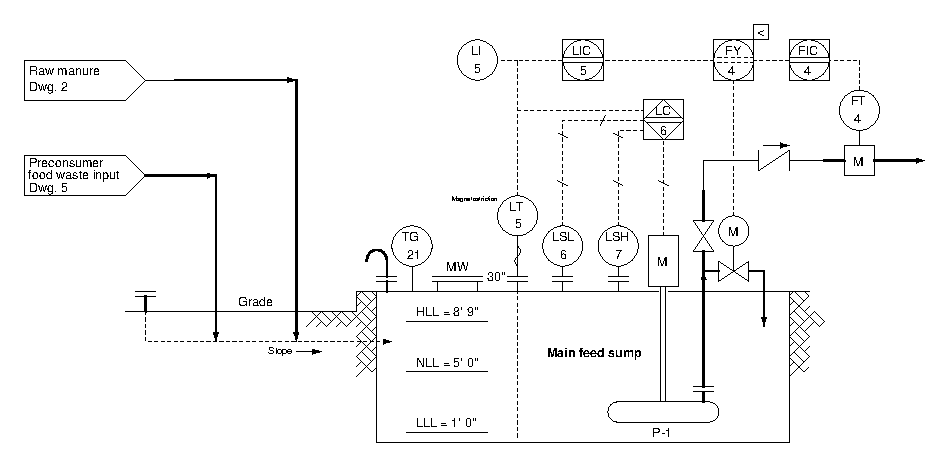
\includegraphics[width=15.5cm]{i00921x05.eps}$$ 

\end{itemize}









\vfil \eject

\noindent
{\bf Labspørsmål}

\vskip 20pt

\begin{itemize}
\item{} Skisser lederkoblinger som gjør dette til et fungerende kontrollsystem. Du skal kun skissere {\it ledninger}, ingen ekstra komponenter er nødvendig:

$$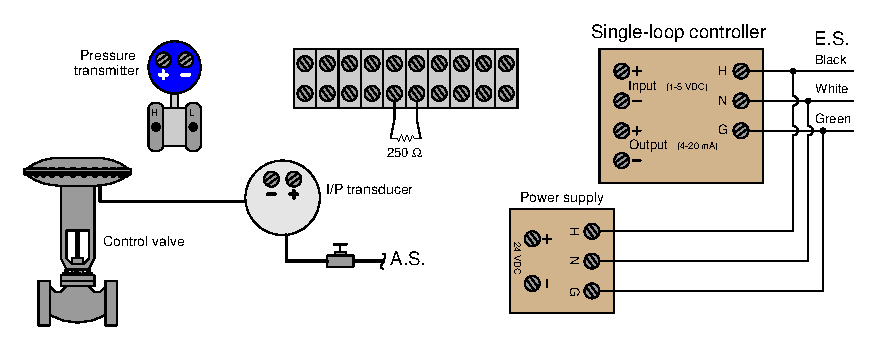
\includegraphics[width=15.5cm]{i00921x07.eps}$$ 

\vskip 20pt

\item{} Beskriv en praktisk anvendelse av {\it feedforward}-regulering og forklar hvordan den virker.

\vskip 20pt

\item{} Beregn pneumatisk trykk i 3-15 PSI-område ved 45 prosent.

\vskip 20pt

\item{} Det er et problem i kontrollsystemet under for matesumpen til en anaerob råtnetank som produserer metangass fra husdyrgjødsel og matavfall. Operatøren rapporterer lav nivåvisning på LI-5 (0 fot 7 tommer), og pumpen (P-1) går ikke. En tekniker foreslår manuell nivåmåling med ``dipstick'' gjennom lufting for å verifisere LI-5. Forklar hva testen forteller om feilens art og plassering dersom (1) målingen bekrefter lavt nivå, og (2) dersom målingen i stedet viser normalt/høyt nivå i uenighet med LI-5:

$$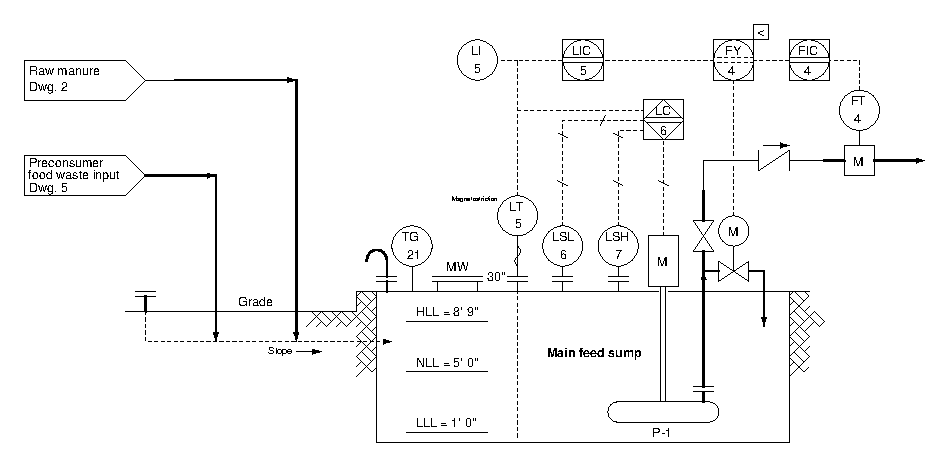
\includegraphics[width=15.5cm]{i00921x05.eps}$$ 

\end{itemize}

%INDEX% Lab exercise, cascade/ratio/feedforward control strategy

%(END_NOTES)
